\documentclass[10pt,border=4pt]{standalone}
\usepackage{mathptmx}
\usepackage{amsmath,amssymb,bm}
\usepackage{tikz}
\usetikzlibrary{patterns,decorations.pathmorphing,decorations.pathreplacing,arrows.meta,fit,backgrounds,calc,positioning,shapes.geometric}
\definecolor{acc}{HTML}{0B5394}
\definecolor{accl}{HTML}{EAF0F7}
\definecolor{grp}{HTML}{F5F5F5}
\definecolor{org}{HTML}{C55A11}
\definecolor{orgl}{HTML}{FBEFE6}
\tikzset{
 dat/.style={draw=black,line width=0.6pt,fill=white,align=center,font=\small,inner sep=3pt,minimum height=0.85cm},
 lay/.style={draw=acc,line width=0.8pt,fill=accl,rounded corners=2pt,align=center,font=\small,inner sep=3pt,minimum height=0.85cm},
 cnd/.style={draw=org,line width=0.8pt,fill=orgl,rounded corners=2pt,align=center,font=\small,inner sep=3pt,minimum height=0.75cm},
 op/.style={circle,draw=black,line width=0.6pt,fill=white,inner sep=0.5pt,font=\small,minimum size=5mm},
 grpb/.style={draw=black!45,dashed,line width=0.6pt,rounded corners=3pt,inner sep=6pt},
 arr/.style={-{Latex[length=2.2mm,width=1.7mm]},line width=0.7pt},
 carr/.style={-{Latex[length=2.2mm,width=1.7mm]},line width=0.7pt,draw=org},
 shp/.style={font=\scriptsize,text=black!70,inner sep=1pt},
 lab/.style={font=\footnotesize,inner sep=1pt},
 ttl/.style={font=\small\bfseries,inner sep=0pt,anchor=west}
}
\newcommand{\xh}{\mathbf{x}_h}\newcommand{\xf}{\mathbf{x}_f}

\tikzset{bx/.style={dat,minimum height=1.1cm,text width=2.9cm,align=center,font=\small}}
\begin{document}\raggedright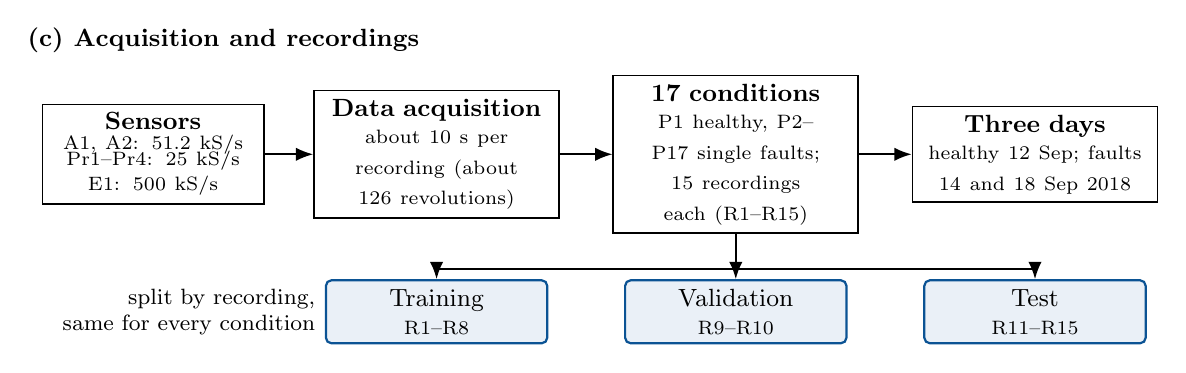
\begin{tikzpicture}[x=1cm,y=1cm]
\node[ttl] at (-1.6,1.45) {(c) Acquisition and recordings};
\node[bx,text width=2.6cm] (s) at (0,0) {\textbf{Sensors}\\[-1pt]\scriptsize A1, A2: 51.2 kS/s\\[-2pt]Pr1--Pr4: 25 kS/s\\[-2pt]E1: 500 kS/s};
\node[bx] (d) at (3.6,0) {\textbf{Data acquisition}\\[-1pt]\scriptsize about 10 s per recording (about 126 revolutions)};
\node[bx] (r) at (7.4,0) {\textbf{17 conditions}\\[-1pt]\scriptsize P1 healthy, P2--P17 single faults; 15 recordings each (R1--R15)};
\node[bx] (p) at (11.2,0) {\textbf{Three days}\\[-1pt]\scriptsize healthy 12 Sep; faults 14 and 18 Sep 2018};
\draw[arr] (s)--(d); \draw[arr] (d)--(r); \draw[arr] (r)--(p);
\node[lay,text width=2.6cm,minimum height=0.8cm] (tr) at (3.6,-2.0) {Training\\[-1pt]\scriptsize R1--R8};
\node[lay,text width=2.6cm,minimum height=0.8cm] (va) at (7.4,-2.0) {Validation\\[-1pt]\scriptsize R9--R10};
\node[lay,text width=2.6cm,minimum height=0.8cm] (te) at (11.2,-2.0) {Test\\[-1pt]\scriptsize R11--R15};
\draw[arr] (r.south)--++(0,-0.45)-|(tr.north); \draw[arr] (r.south)--(va.north); \draw[arr] (r.south)--++(0,-0.45)-|(te.north);
\node[lab,anchor=east,align=right] at (2.1,-2.0) {split by recording,\\same for every condition};
\end{tikzpicture}\end{document}
